\documentclass{scrartcl}

\usepackage{ucs}
\usepackage[utf8x]{inputenc}
\usepackage[english]{babel}
\usepackage{graphicx}
\usepackage{amsmath}
\usepackage{amssymb}
\usepackage{hyperref}
\usepackage{blkarray}
\usepackage{tabulary}

\setlength\parindent{0pt}

\newcommand{\norm}[1]{\left\lVert#1\right\rVert}

\title{Maschinelles Lernen \\ Zusammenfassung}
\author{Thomas Mohr}
\date{}

\begin{document}
\maketitle
\pagebreak
\tableofcontents
\pagebreak

\section{Grundlagen}

\subsection{(Un)-überwachtes Lernen}

\begin{itemize}
	\item Eine \textbf{überwachte} Lernaufgabe liegt vor, wenn wir Beispiele 
	haben, die das zu lernende Attribut bereits tragen (Zielvariable).
	\begin{itemize}
		\item \textbf{Regression} im Fall von kontinuierlichen Werten (z.B. $ 
		\mathbb{R} $) - eigentlich numerisch
		\item \textbf{Klassifikation} im Fall von diskreten Labeln (z.B. 
		\textit{TRUE, FALSE}; ausgezeichnet, durchschnittlich, schlecht) - 
		eigentlich nominal oder ordinal
	\end{itemize}
	\item Eine \textbf{unüberwachte} Lernaufgabe liegt vor, wenn es kein 
	Attribut gibt, das wir lernen wollen und für das wir bereits Beispiele 
	haben.
	\begin{itemize}
		\item Clustering, also die Unterteilung der Daten in eine Menge 
		von Gruppen
		\item Finden von Ausreißern
	\end{itemize}
\end{itemize}

\subsection{Inkrementelles Lernen}

\begin{itemize}
	\item Anstatt das Modell stets von Null an zu lernen, wird das alte Modell 
	mit neuen Beispielen erweitert.
\end{itemize}

\subsection{Aktives Lernen}

\begin{itemize}
	\item Aktive Lernverfahren erzeugen die Beispiele selbst, d.h., sie sagen 
	dem Benutzer, welches Tupel benötigt wird.
\end{itemize}

\subsection{Data cleansing}

\begin{itemize}
	\item Fehlende Werte auffüllen
	\item Rauschen aus den Daten entfernen
	\item Daten glätten
	\item Ausreißer entfernen
	\item Identische Tupel identifizieren
	\item Daten komprimieren
\end{itemize}

\subsection{Datensatz}

\begin{itemize}
	\item Ein Datensatz ist eine Tabelle.
	\item Eine Instanz (auch Objekt) ist eine Zeile in dieser Tabelle.
	\item Ein Attribut ist ein Feld, das ein Merkmal des Objekts repräsentiert. 
	Mögliche Arten von Attributen sind:
	\begin{itemize}
		\item nominal (kategorisch)
		\begin{itemize}
			\item Keine sinnvolle Ordnung
			\item Wir können nicht rechnen (z.B. Mittelwert, Median, Abstände).
		\end{itemize}
		\item ordinal (sortierte Kategorien)
		\begin{itemize}
			\item Sinnvolle Ordnung
			\item Der Unterschied zwischen zwei Ausprägungen ist i.d.R. 
			unbekannt.
		\end{itemize}
		\item binär
		\begin{itemize}
			\item Können nur zwei Werte annehmen
		\end{itemize}
		\item numerisch
		\begin{itemize}
			\item Messbare Quantitäten
			\item Abstand zwischen zwei Werten kann quantifiziert werden.
			\item Auf den Attributen kann gerechnet werden.
			\item Wir unterscheiden:
			\begin{itemize}
				\item diskrete Attribute (endliche oder abzählbar unendliche 
				Menge von womöglichen Ausprägungen)
				\item kontinuierliche Werte, reele Zahlen
				\item Attribute mit echtem Nullpunkt (Gewicht, Größe)
				\item Attribute ohne echten Nullpunkt (Jahresangaben, 
				Temperatur in °C)
			\end{itemize}
		\end{itemize}
	\end{itemize}
	\item Ein Datensatz besitzt $ N $ Instanzen und $ d $ Attribute.
	\begin{itemize}
		\item $ x_i $ beschreibt die $ i $-te Instanz.
		\item $ x_{ij} $ beschreibt das $ j $-te Attribut der $ i $-ten Instanz.
		\item $ x $ beschreibt einen $ d $-dimensionalen Vektor.
		\item Liegt eine überwachte Lernaufgabe vor, so ist das Label der $ i 
		$-ten Instanz $ t_i $.
	\end{itemize}
\end{itemize}

\pagebreak
\section{Deskriptive Statistik}

\subsection{Beschreibung von Daten}

\begin{itemize}
	\item Wir betrachten nun Spalten des Datensatzes, also z.B. Spalte $ j $:
	\[ X_j = (x_{1j},\ldots,x_{Nj}) \]
\end{itemize}

\subsection{Mittelwert}

\begin{itemize}
	\item Der Erwartungswert (Mittelwert) macht Aussagen zur Lage (dem 
	''Zentrum'') der Daten:
	\[ \mu_j := \sum_{i=1}^{N} x_{ij} \cdot p(x_{ij}) = \frac{1}{N} 
	\sum_{i=1}^{N} x_{ij} \]
	\item Ist eine Gewichtung vorhanden, so kann der gewichtete 
	\underline{Mittelwert} herangezogen werden:
	\[ \mu'_j := \frac{\sum_{i=1}^{N} w_i x_{ij}}{\sum_{i=1}^{N} w_i} \]
	\item Problematisch bei Ausreißern
\end{itemize}

\subsection{Median und Midrange}

\begin{itemize}
	\item Der Median ist der mittlere Wert in der \underline{sortierten} Folge 
	$ X_j $.
	\item Das mittlere Element muss nicht existieren.
	\begin{itemize}
		\item Per Definition wählen wir dann als Median den Wert
		\[ \frac{1}{2} (x_{\frac{N}{2},j} + x_{\frac{N}{2+1},j}) \]
		im Fall numerischer Daten.
		\item Im Fall von ordinalen Daten kann der Median das \underline{linke} 
		oder das \underline{rechte} Element sein, oder jede mögliche Ausprägung 
		dazwischen.
	\end{itemize}
	\item Der Midrange ist das arithmetische Mittel von Maximum und Minimum von 
	$ X_j $.
\end{itemize}

\subsection{Modus}

\begin{itemize}
	\item Der Modus ist die am häufigsten vorkommende Ausprägung. Somit ist der 
	Modus auch für nominale Attribute berechenbar.
	\item Wird die maximale Häufigkeit für mehr als einen Wert angenommen, so 
	gibt es mehr als einen Modus.
	\item Kommt jede Ausprägung maximal einmal vor, so ist der Modus nicht 
	existent.
\end{itemize}

\subsection{Varianz und Schiefe}

\begin{itemize}
	\item Über einen Vergleich von Modus, Median und Mittelwert können wir 
	(erste) Aussagen zur Schiefe machen.
	\item Über Maximum und Minimum können wir die Ausbreitung bestimmen.
	\item Mit dem Moment 2-ter und 3-ter Ordnung können wir beides auch 
	quantisieren.
	\item Das Moment $ k $-ter Ordnung des $ j $-ten Attributs ist definiert 
	als:
	\[ m_j^{(k)} = E((X_j - \mu_j)^k) \]
	mit $ E(X) = \sum_{1 \leq i \leq N} x_{ij} p(x_{ij}) $ und $ \mu_j $ ist 
	Erwartungswert von $ X_j $
\end{itemize}

\subsubsection{Moment $ k $-ter Ordnung}

\begin{itemize}
	\item $ k=1:? $
	\item $ k=2:Var(X_j) := E((X_j - \mu_j)^2) = E(X_j^2) - \mu_j^2 $
	\[  \]
	\begin{itemize}
		\item Die Varianz gibt die erwartete quadratische Abweichung vom 
		Mittelwert an.
		\item Sie ist also ein Maß für die Streuung der Daten (um den 
		Mittelwert).
		\item Die Quadratwurzel der Varianz wird als Standardabweichung 
		bezeichnet und mit $ \sigma $ symbolisiert.
	\end{itemize}
	\item $ k=3:v(X_j) := E((X_j - \mu_j)^3) $
	\begin{itemize}
		\item Die Schiefe ist eine Kennzahl für die Asymmetrie einer Verteilung:
		\[ v(X) = \frac{3(\overline{X} - \tilde{X})}{s} \]
		\item $ v(X_j) < 0 $: Verteilung ist linksschief
		\item $ v(X_j) > 0 $: Verteilung ist rechtsschief
		\item $ v(X_j) = 0 $: Verteilung symmetrisch
	\end{itemize}
	\item $ k=4:w(X_j) := E((X_j - \mu_j)^4) $
	\begin{itemize}
		\item Die Kurtosis ist eine Kennzahl für die Wölbung einer Verteilung:
		\[ w(X) = \frac{1}{N} \sum_{i=1}^{N} (\frac{x_i - \overline{X}}{s})^4 \]
		\item $ w(X) < 0 $: Verteilung ist platykurtisch (flachgipflig)
		\item $ w(X) > 0 $: Verteilung ist leptokurtisch (steilgipflig)
		\item $ w(X) = 0 $: Verteilung ist mesokurtisch (normalgipflig)
	\end{itemize}
\end{itemize}

\subsection{Quantil}

\begin{itemize}
	\item Zur Berechnung der Quantile wird $ X_j $ zunächst aufsteigend 
	sortiert.
	\item Das $ k $-te Quantil ist der Wert $ x $ aus $ X_j $, so dass maximal 
	$ \frac{k}{q} $ der Werte in $ X_j $ kleiner als $ x $ sind, und $ 
	\frac{(q-k)}{q} $ größer; für $ 0<k<q $.
	\item Es gibt somit $ (q-1) $ $ q $-Quantile.
	\item Sei $ p := \frac{k}{q} $. Dann ist das $ k $-te $ q $-Quantil von $ 
	X_j $ definiert als:
	\[ x_{pj} := \begin{cases}
		\frac{1}{2} (x_{Np} + x_{Np+1}) & Np \text{ gerade} \\
		x_{\lfloor Np+1 \rfloor} & Np \text{ ungerade}
	\end{cases} \]
\end{itemize}

\subsubsection{Interquantile range (IQR)}

\begin{itemize}
	\item Ist definiert als $ IQR = Q3 - Q1 $
	\item Es gibt an, wie die 50\% der mittleren Daten streuen
	\item Der IQR kann zudem benutzt werden, um Ausreißer zu erkennen.
	\begin{itemize}
		\item Berechne $ \Delta = 1.5 \cdot IQR $
		\item Ein Ausreißer ist ein Wert, der
		\begin{itemize}
			\item kleiner $ Q1 - \Delta $ ist.
			\item größer $ Q3 + \Delta $ ist.
		\end{itemize}
	\end{itemize}
	\item $ Q1,Q2,Q3,IQR $ sowie Minimum und Maximum können graphisch im 
	Boxplot zusammengefasst werden.
\end{itemize}

\subsection{Korrelation zwischen Attributen}

\begin{itemize}
	\item Wir betrachten nun einen (möglichen) Zusammenhang der Spalten $ X_i $ 
	und $ X_j $.
	\item Je nach Attribut existieren unterschiedliche Maße:
	\begin{itemize}
		\item Korrelationskoeffizienten und Varianz für numerische Daten
		\item Rangkorrelationskoeffizienten für ordinale Daten
		\item $ \chi^2 $-Test für nominale Attribute
	\end{itemize}
\end{itemize}

\subsubsection{Kovarianz für numerische Daten}

\begin{itemize}
	\item Erlaubt zu messen, wie startk sich zwei Variablen gemeinsam ändern
	\item Wir benötigen den Begriff des Erwartungswerts, der hier aber dem 
	Mittelwert entspricht:
	\[ E(X_j) = \overline{X_j} = \frac{1}{N} \sum_{i=1}^{N} x_{ij} \]
	\item $ Cov(X_i,X_j) = E((X_i - \overline{X_i})(X_j - \overline{X_j})) = 
	E(X_iX_j) - \overline{X_i} \cdot \overline{X_j} $
	\item Tendieren $ X_i $ und $ X_j $ dazu sich gemeinsam zu ändern, so ist $ 
	Cov(X_i,X_j) $ positiv, bei entgegengesetzter Änderung negativ.
	\item Das Maß ist nicht normalisiert.
\end{itemize}

\subsubsection{Korrelationskoeffizienten für numerische Daten}

\begin{itemize}
	\item Der Korrelationskoeffizient ist normalisiert im Interval $ [-1,1] $:
	\[ cor(X_i,X_j) = \frac{Cov(X_i,X_j)}{\sqrt{Var(X_i)} \sqrt{Var(X_j)}} \]
	\item Wir haben keine Korrelation bei einem Wert von 0.
	\item Positive (negative) Korrelation liegt bei positiven (negativen) 
	Werten vor.
\end{itemize}

\subsubsection{Rangkorrelationskoeffizient}

\begin{itemize}
	\item Der (Spearman) Rangkorrelationskoeffizient basiert auf den Rängen der 
	Elemente; wir betrachten die Spalten $ X_i $ und $ X_j $. Er wird berechnet 
	als:
	\[ r_s(X_i,X_j) = \frac{\sum_{1 \leq k \leq N} (rank(x_{ki}) - 
	\mu Rank(X_i)) \cdot (rank(x_{kj}) - \mu Rank(X_j)}{\sqrt{\sum_{1 \leq k 
	\leq N} (rank(x_{ki}) - \mu Rank(X_i))^2} \sqrt{\sum_{1 \leq k \leq N} 
(rank(x_{kj}) - \mu Rank(X_j))^2}} \]
	mit $ \mu Rank(X_i) $ ist der mittlere Rang in Spalte $ i $
	\item Der Rang wird aufsteigend anhand der Werte bestimmt. Der kleinste 
	Wert nimmt dabei Rang 1 ein, der zweitkleinste Rang 2, usw. Tritt ein Wert 
	mehrfach auf, so ergibt sich der Rang aus dem Arithmetischen Mittel.
	\item $ rs $ ist normalisiert in $ [-1,1] $.
\end{itemize}

\subsubsection{$ \chi^2 $-Test}

\begin{itemize}
	\item Seien $ a_1,\ldots,a_c $ die $ c $ Werte, die das Attribut $ X_k $ 
	aufweist, $ b_1,\ldots,b_r $ die $ r $ Werte, die wir in der Spalte $ X_l $ 
	finden.
	\item Berechne in $ o_{ij} $ die beobachtete Anzahl der Ereignisse, dass $ 
	X_k $ den Wert $ a_i $ und $ X_l $ den Wert $ b_j $ \underline{gemeinsam} 
	annehmen.
	\item Wir können auch die erwartete Anzahl berechnen (für nicht korrelierte 
	Atrribute):
	\[ e_{ij} = \frac{1}{N} (|X_k=a_i| \cdot |X_l=b_j|) \]
	\item Die Pearson $ \chi^2 $ Statistik kann wie folgt berechnet werden:
	\[ \chi^2 = \sum_{i=1}^{c} \sum_{j=1}^{r} \frac{(o_{ij} - 
	e_{ij})^2}{e_{ij}} \]
	\item Die Statistik testet die \underline{Null-Hypothese der 
	Unabhängigkeit} zweier Variablen.
	\item Der Test basiert auf einem Signifikanzniveau mit $ (r-1) \cdot (c-1) 
	$ Freiheitsgraden.
	\begin{itemize}
		\item Das Signifikanzniveau ist die Wahrscheinlichkeit, mit der die 
		Nullhypothese fälschlicherweise verworfen wird kann, obwohl sie 
		eigentlich richtig ist.
	\end{itemize}
	\item Die Hypothese kann abgelehnt werden, wenn der Wert der Prüfgröße 
	größer ist als das $ (1-a) $-Quantil der $ \chi^2 $ Verteilung.
\end{itemize}

\subsection{Visualisierung}

\subsubsection{Boxplots}

\begin{itemize}
	\item $ IQR $ ist die breite Mitte der Box.
	\item Das untere Quartil ($ X_{0,25} $) ist die untere/linke Kante der Box.
	\item Das obere Quartil ($ X_{0,75} $) ist die obere/rechte Kante der Box.
	\item Der Median ist durch eine Linie in der Box gekennzeichnet.
	\item Die langen Enden der Box heißen Whisker und geben die Grenzen für 
	Ausreißer an. Alle Werte die außerhalb der Whisker, und damit des 
	zulässigen Bereichs liegen, heißen Ausreißer.
\end{itemize}

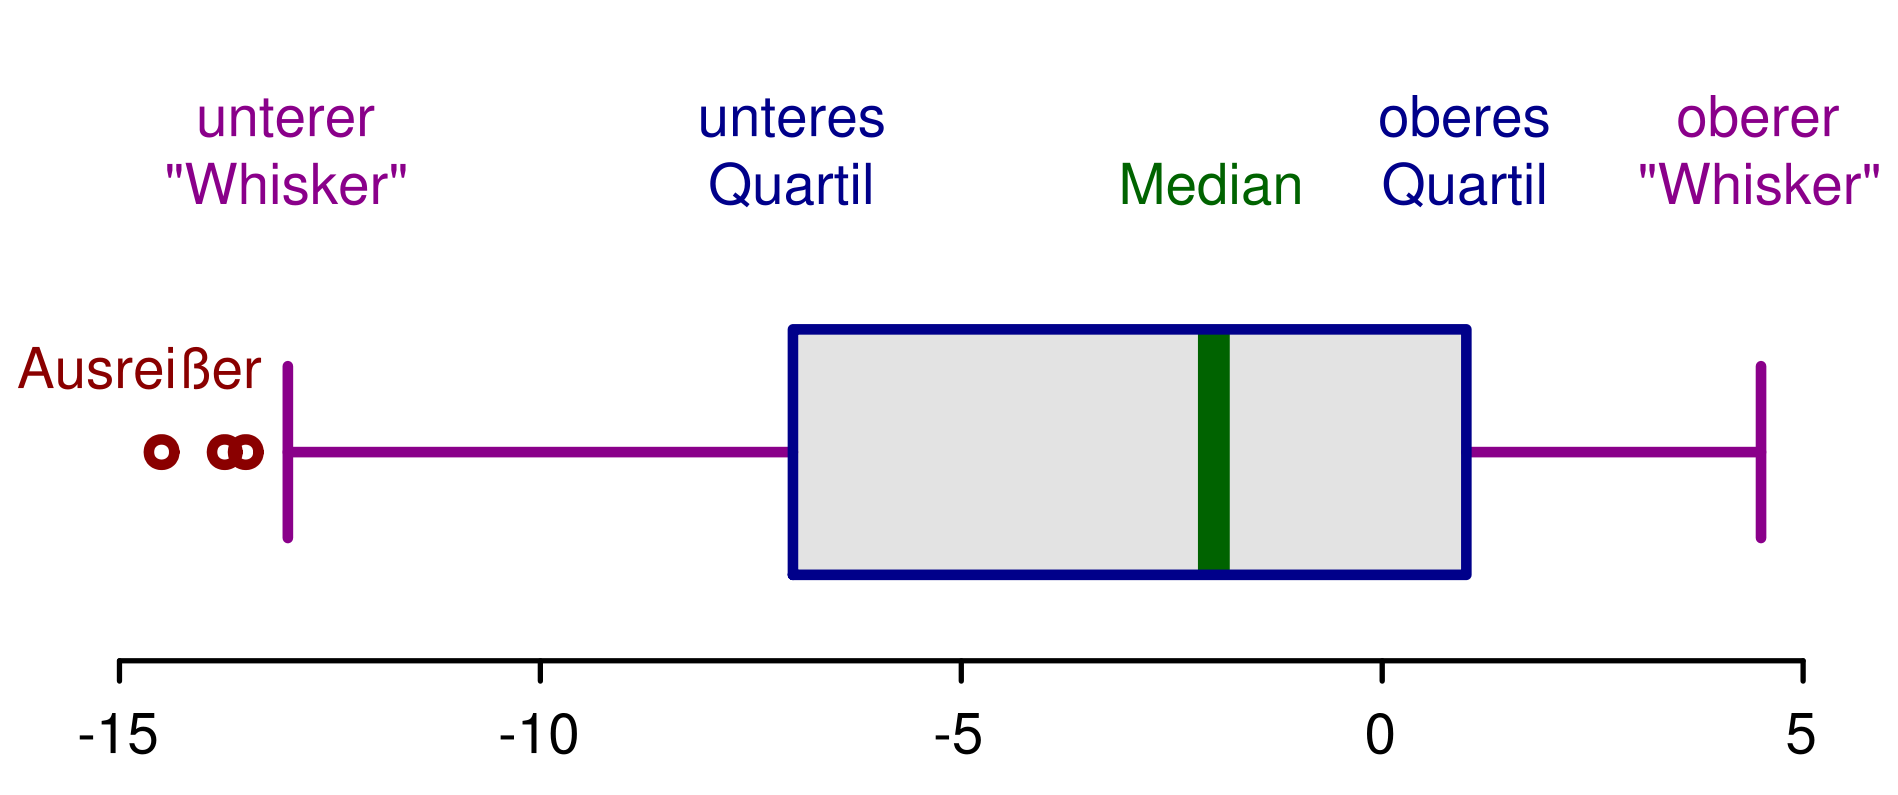
\includegraphics[width=\linewidth]{figures/boxplot.png}

\subsubsection{Histogramme}

\begin{itemize}
	\item Werden zur Darstellung von Häufigkeitsverteilungen verwendet.
	\item Bei numerischen Attributen müssen disjunkte Klassen definiert werden.
	\begin{itemize}
		\item Die Balkenbreite kann durch zwei Verfahren bestimmt werden:
		\begin{itemize}
			\item Scott-Regel: $ w = \dfrac{3,49 \cdot \sigma}{\sqrt[3]{N}} $
			\item Regel von Diaconis: $ w = \frac{2(Q3-Q1)}{\sqrt[3]{N}} $
		\end{itemize}
		\item Die Häufigkeit ist proportional zum Flächeninhalt.
	\end{itemize}
\end{itemize}

\paragraph{Beispiel}

\begin{center}
	\tymin=35pt
	\begin{tabulary}{\linewidth}{|C|C|C|C|C|}
		\hline 
		Klasse $ j $ & Zahl der PKW pro 1000 & Anzahl der Länder (absolute 
		Häufigkeit) $ n_j $ & Klassenbreite $ d_j $ & Rechteckshöhe 
		(Häufigkeitsdichte) $ h_j = \frac{n_j}{h_j} $ \\ 
		\hline 
		1 & $ 0-200 $ & 5 & 200 & 0,025 \\ 
		\hline 
		2 & $ 200-300 $ & 6 & 100 & 0,06 \\ 
		\hline 
		3 & $ 300-400 $ & 6 & 100 & 0,06 \\ 
		\hline 
		4 & $ 400-500 $ & 9 & 100 & 0,09 \\ 
		\hline 
		5 & $ 500-700 $ & 6 & 200 & 0,03 \\ 
		\hline 
		Summe $ \sum $ &  & 32 &  &  \\ 
		\hline 
	\end{tabulary} 
\end{center}

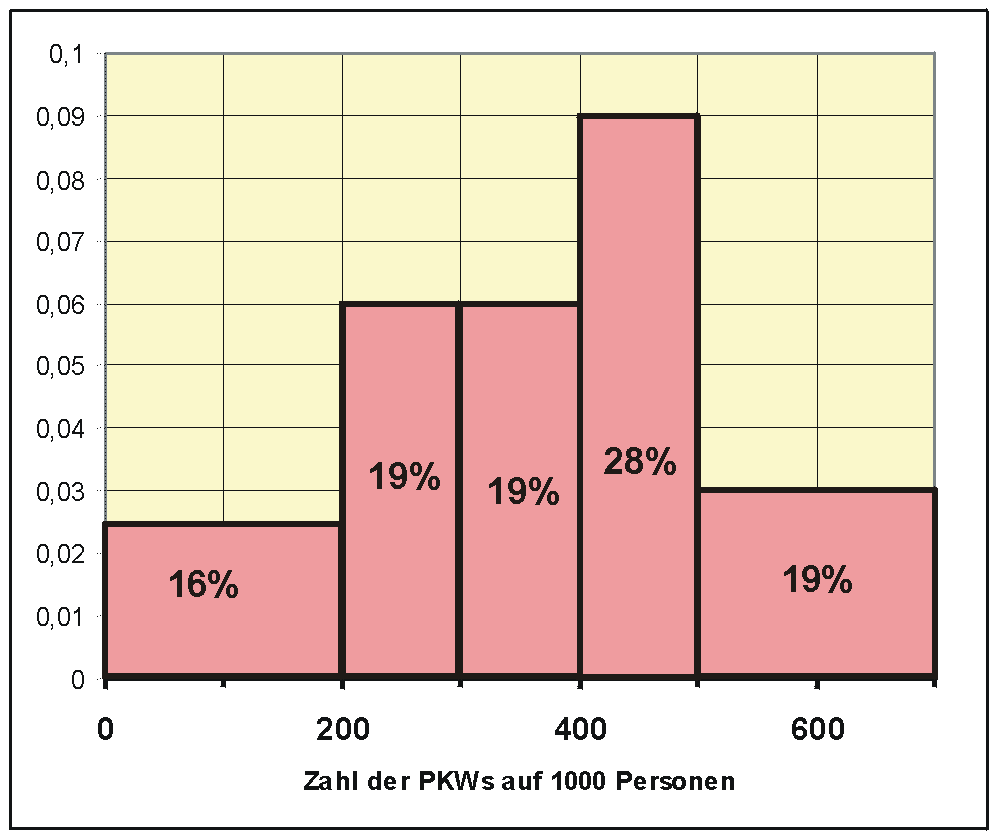
\includegraphics[width=\linewidth]{figures/hist.png}

\subsubsection{Quantil-Plots}

\begin{itemize}
	\item Ein Quantil-Plot erlaubt es das Verhalten der Werte eines Attributs 
	abzuschätzen.
	\item Die Daten im $ i $-ten Attribut werden sortiert und das $ k $-te 
	Element wird abgetragen auf $ f_k = \frac{k-0,5}{N} $.
\end{itemize}

\paragraph{Quantil-Quantil-Plots (qq-Plots)}

\begin{itemize}
	\item Die Quantile einer Verteilung werden gegen die Quartile einer anderen 
	Verteilung abgetragen.
	\item Die Werte in werden in den Attributen $ X_i $ und $ X_j $ sortiert.
	\item Enthalten beide Attribute die gleiche Anzahl an Elementen, so wird $ 
	x_{ki} $ auf $ x_{kj} $ mit $ 1 \leq k \leq N $ abgebildet.
	\item Ansonsten ist $ |X_i| < |X_j| $ und nur $ |X_i| $ Punkte können 
	geplottet werden:
	\begin{itemize}
		\item $ x_{ki} $ ist das $ \frac{k-0,5}{|X_i|} $ Quantil.
		\item Das $ \frac{k-0,5}{|X_i|} $ Quantil von $ X_j $ muss dann 
		interpoliert werden.
	\end{itemize}
\end{itemize}

\subsection{Distanzen}

\begin{itemize}
	\item Ähnlichkeits- oder Distanzmaß, dass ein Objekt-Paar auf einen 
	numerischen Wert abbildet
	\item Metrik:
	\begin{itemize}
		\item Identität: $ d(x_i,x_j) = 0 \iff x_i = x_j $
		\item Symmetrie: $ d(x_i,x_j) = d(x_j,x_i) $
		\item Dreiecksungleichung: $ d(x_i,x_j) \leq d(x_i,x_k) + d(x_k,x_j) $
		\item $ d(\cdot,\cdot) $ beschreibt hier ein Funktion und ist nicht mit 
		der Anzahl an Attributen zu verwechseln.
	\end{itemize}
	\item Eine Distanz kann in eine Ähnlichkeit und umgekehrt umgewandelt 
	werden. Ist $ d: 0 \times 0 \rightarrow [0,1] $, so kann $ s(x_i,x_j) = 1 - 
	d(x_i,x_j) $ definiert werden.
\end{itemize}

\subsubsection{Distanz auf numerischen Attributen}

\begin{itemize}
	\item Minkowski Abstand (Metrik)
	\[ d_h(x_i,x_j) = \sqrt[h]{|x_{i1} - x_{j1}|^h + \ldots + |x_{id} - 
	x_{jd}|^h} \]
	\begin{itemize}
		\item $ h=1 $: Manhattan Distanz
		\item $ h=2 $: Euklidische Distanz
		\item Supremum Distanz für $ h \rightarrow \inf $, die zu $ \max_{1 
		\leq f \leq d} |x_{if} - x_{jf}| $ konvergiert
	\end{itemize}
\end{itemize}

\subsubsection{Distanz auf ordinalen Attributen}

\begin{itemize}
	\item Betrachtung der Ränge und einer darauf basierenden Abbildung.
	\item Sei $ M_f $ die Menge möglicher Ränge für das Attribut $ f $.
	\item Ersetze Wert $ x_{if} $ durch dessen Rang $ r_{if} \in \{ 
	1,\ldots,M_f \} $.
	\item Nun kann mit den Rängen gearbeitet werden, allerdings sollte zuvor 
	normalisiert werden:
	\[ z_{if} = \frac{r_{if} - 1}{M_f - 1} \in [0,1] \]
	\item Die $ z_{if} $ sind numerisch und können beispielsweise mit der 
	Minkowski Distanz verglichen werden.
\end{itemize}

\subsubsection{Distanz auf nominalen Attributen}

\begin{itemize}
	\item Werden Objekte durch $ d $ nominale Attribute beschrieben, so kann 
	die Distanz zwischen $ x_i $ und $ x_j $ wie folgt berechnet werden
	\[ d(x_i,x_j) = \frac{d-m}{d} \]
	wobei $ m $ die Anzahl der Übereinstimmungen ist.
\end{itemize}

\subsubsection{Distanz auf binären Attributen}

\begin{center}
	\begin{tabular}{|c|c|c|c|}
		\hline
		& 1 & 0 & $ \sum $ \\ 
		\hline
		1 & $ q $ & $ r $ & $ q+r $ \\ 
		\hline
		0 & $ s $ & $ t $ & $ s+t $ \\ 
		\hline
		$ \sum $ & $ q+s $ & $ r+t $ & $ d $ \\
		\hline
	\end{tabular} 
\end{center}

\begin{itemize}
	\item Je nachdem, ob Attribute symmetrisch sind, können zwei verschiedene 
	Distanzen definiert werden.
	\begin{itemize}
		\item Ist sowohl der Zustand ''0'' als auch ''1'' gleichwertig, so 
		definieren wir die Distanz als:
		\[ d(x_i,x_j) = \frac{r+s}{d} \]
		\item Im Fall eines asymmetrischen Attributs tragen die ''1''-en die 
		tatsächliche Information; ''0''-en sind nicht von Interesse:
		\[ d)(x_i,x_j) = \frac{r+s}{q+r+s} \]
		\item Der Jaccard-Koeffizient ist ein häufig vorkommendes 
		\underline{Ähnlichkeitsmaß}:
		\[ s(x_i,x_j) = 1 - d(x_i,x_j) = \frac{q}{q+r+s} \]
	\end{itemize}
\end{itemize}

\subsubsection{Distanz auf gemischten Typen}

\begin{itemize}
	\item Sei $ d $ die Anzahl unterschiedlicher Attributstypen:
	\[ d(x_i,x_j) = \frac{\sum_{f=1}^{d} \delta_{ij}^{(f)} \frac{|x_{if} - 
	x_{jf}|}{\max_{1 \leq h \leq N} x_{hf} - \min_{1 \leq h \leq N} 
	x_{hf}}}{\sum_{f=1}^{d} \delta_{ij}^{(f)}} \]
	\item $ \delta_{if}^{(f)} $ ist ein binärer Indikator.
	\begin{itemize}
		\item Er ist 0, falls ($ x_{if} $ oder $ x_{jf} $ unbekannt sind, oder 
		wenn) $ x_{if} = x_{jf} = 0 $ und das binäre Attribut $ f $ 
		asymmetrisch ist; ansonsten ist $ \delta_{if}^{(f)} = 1 $.
	\end{itemize}
\end{itemize}

\subsection{Dimensionsreduktion und Einbettung in den Vektorraum}

\subsubsection{Multidimensionale Skalierung}

\begin{itemize}
	\item Überführung von Punkten aus einem $ d $-dimensionalen Raum in einen $ 
	m $-dimensionalen Raum $ (d > m) $ oder metrischer Raum in Vektorraum.
	\item Die paarweisen Euklidischen Abstände sollen dabei möglichst wenig 
	verändert werden.
	\item Es gilt:
	\begin{align*}
		d(x_i,x_j)^2 &= d_{ij}^2 = \sum_{k=1}^{d} (x_{ik} - x_{jk})^2 \\
		&= \underbrace{\sum_{k=1}^{d} (x_{ik})^2}_{b_{ii}} - 2 
		\underbrace{\sum_{k=1}^{d} x_{ik} x_{jk}}_{b{ij}} + 
		\underbrace{\sum_{k=1}^{d} (x_{jk})^2}_{b_{jj}} \\
		&= b_{ii} + b_{jj} - 2b_{ij}
	\end{align*}
	\item Zentriere Daten im Urpsrung: $ \sum_{i=1}^{N} x_{ij} = 0 \quad 
	\forall j = 1,\ldots,d $
	\item Die $ b_{ij} $ können zu einer $ (N \times N) $-Matrix $ B $ 
	zusammengefasst werden. Daher gilt $ B=XX^T $.
	\item $ X $ ist die gesuchte Matrix, die den Datensatz durch $ N $ 
	Attribut-Vektoren beschreibt und die es nun zu approximieren gilt.
	\item Spektrale Zerlegung:
	\[ X = CD^{\frac{1}{2}} \]
	mit $ C $ ist die Matrix, deren Spalten den Eigenvektoren von $ B $ 
	entsprechen; $ D $ ist eine diagonale Matrix mit den Eigenwerten.
\end{itemize}

\subsection{Hauptkomponentenanalyse}

\begin{itemize}
	\item Die Hauptkomponentenanalyse (PCA) projiziert ein Objekt $ x \in 
	\mathbb{R}^d $ auf $ z \in \mathbb{R}^d $ wie folgt:
	\[ z=w^Tx \]
	\item Ziel ist es durch eine Projektion die Varianz auf den neuen 
	Attributen $ Z_1,\ldots,Z_d $ zu maximieren.
	\item Tatsächlich beträgt dabei die Korrelation zwischen allen Paaren $ 
	(Z_i,Z_j) $ auch 0.
	\item Gesucht ist ein neuer $ m (<d) $ dimensionaler Raum, auf dem die 
	Daten mit minimalem Informationsverlust projiziert werden können.
\end{itemize}

\section{Regression}

\begin{itemize}
	\item Es liegen numerische Daten vor.
	\item Es existiert eine Zielvariable, die wir aus den anderen hervorgesagt 
	werden soll.
	\item Ein Modell
	\[ f: \mathbb{R}^d \rightarrow \mathbb{R} \]
	soll gelernt werden.
	\item Das Problem wird als
	\begin{itemize}
		\item univariat bezeichnet, falls $ d=1 $.
		\item multivariat bezeichnet, falls $ d>1 $.
	\end{itemize}
	\item Ein Modell $ y(x) $ muss bewertet werden können.
	\item Dazu wird eine Fehlerfunktion $ L: \mathbb{R} \times \mathbb{R} 
	\rightarrow \mathbb{R} $ benötigt, die den Fehler auf den zukünftigen 
	Eingaben misst.
	\item Eine gängige Wahl für die Regression ist der quadratische Fehler:
	\[ (y(x), t) \rightarrow (y(x) - t)^2 \]
	\item Das Risiko (der erwartete Fehler) kann somit wie folgt angegeben 
	werden:
	\[ R(y) = E[L] = \int L(t, y(x)) dP(x,t) \]
	\item Dieses Risiko kann jedoch nicht berechnet werden.
\end{itemize}

\subsection{Bewertung und Fehler}

\begin{itemize}
	\item Die Approximation $ R(y) = \int L(t, y(x)) dP(x,t) $ führt zum 
	\underline{empirischen Risiko}:
	\begin{align*}
		R_{emp}(y) &= \frac{1}{N} \sum_{i=1}^{N} L(y(x_i), t_i) \\
		&= \frac{1}{N} \sum_{i=1}^{N} (y(x_i) - t_i)^2
	\end{align*}
	\item Dieser Ausdruck kann ausgewertet werden. Es wird eine Funktion (ein 
	Modell) $ y: \mathbb{R}^d \rightarrow \mathbb{R} $ gesucht, die das 
	empirische Risiko minimiert.
\end{itemize}

\subsubsection{Fitten eines Polynoms}

\begin{itemize}
	\item Nun wird der multivariate Fall betrachtet ($ x_{i0} = 1 $ für $ 1 
	\leq i \leq N $).
	\begin{itemize}
		\item Somit wird eines neues Attribut $ X_0 $ hinzugefügt, mit Wert 1 
		für jede Instanz.
		\[
			\begin{blockarray}{ccc}
				X_0 & \ldots & X_d \\
				\begin{block}{(ccc)}
					1 & \ldots & x_{1d} \\
					\vdots & \ddots & \vdots \\
					1 & \ldots & x_{Nd} \\
				\end{block}
			\end{blockarray}
		\]
		\begin{align*}
			y(x_i, w) &= w_0x_{i0} + w_1x_{i1} + w_2x_{i2} + \ldots + w_dx_{id} 
			\\
			&= \sum_{j=0}^{d} w_jx_{ij}
		\end{align*}
	\end{itemize}
	\item Nun muss das optimale $ w $ gefunden werden, also jenes, für das
	\[ R_{emp}(w) = \frac{1}{N} \sum_{i=1}^{N} L(y(x_i), t_i) \]
	minimiert wird.
	\item Gesucht wird also $ w^* = A^{-1} y $ mit:
	\[ A = \begin{pmatrix}
		\sum_{i} x_{i0}x_{i0} & \sum_{i} x_{i1}x_{i0} & \sum_{i} 
		x_{i2}x_{i0} & \ldots & \sum_{i} x_{id}x_{i0} \\
		\sum_{i} x_{i0}x_{i1} & \sum_{i} x_{i1}x_{i1} & \sum_{i} 
		x_{i2}x_{i1} & \ldots & \sum_{i} x_{id}x_{i1} \\
		\vdots & \vdots & \vdots & \ddots & \vdots \\
		\sum_{i} x_{i0}x_{id} & \sum_{i} x_{i1}x_{id} & \sum_{i} 
		x_{i2}x_{id} & \ldots & \sum_{i} x_{id}x_{id}
	\end{pmatrix} \]
	\[ w = \begin{pmatrix}
		w_0 \\
		w_1 \\
		w_2 \\
		\vdots \\
		w_d
	\end{pmatrix} \]
	\[ y = \begin{pmatrix}
		\sum_i t_i x_{i0} \\
		\sum_i t_i x_{i1} \\
		\sum_i t_i x_{i2} \\
		\vdots \\
		\sum_i t_i x_{id} \\
	\end{pmatrix} \]
	\item Die Berechnung kann effizienter gestaltet werden durch $ w^* = 
	(D^TD)^{-1} D^Tt $ mit:
	\[ D = \begin{pmatrix}
		x_{i0} & x_{11} & x_{12} & \ldots & x_{1d} \\
		x_{i0} & x_{21} & x_{22} & \ldots & x_{2d} \\
		\vdots & \vdots & \vdots & \ddots & \vdots \\
		x_{i0} & x_{N1} & x_{N2} & \ldots & x_{Nd} \\
	\end{pmatrix} \]
	\[ t = \begin{pmatrix}
		t_1 \\
		t_2 \\
		t_3 \\
		\vdots \\
		t_N
	\end{pmatrix} \]
\end{itemize}

\subsection{Overfitting}

\begin{itemize}
	\item Es wird nicht nur das durch die Daten zugrundeliegende Modell, 
	sondern auch das Rauschen, gelernt.
	\item Jedoch soll ein Modell erzeugt werden, das gut 
	\underline{generalisiert}.
	\item Es kann ein Regularisierungsterm verwendet werden, um hohe 
	Koeffizienten zu bestrafen:
	\[ R'(w) = \frac{1}{2} \sum_{i=1}^{N} (y(x_i,w) - t_i)^2 + 
	\frac{\lambda}{2} \norm{w}^2 \]
	\item Ein $ \lambda = 0 $ führt zu dem alten Ansatz; je größer $ \lambda $, 
	desto stärker werden hohe Koeffizienten bestraft.
	\item Es soll eine gute \underline{Generalisierung} erreicht werden, 
	demzufolge muss
	\[ \int L(t, y(x)) dP(x,t) \]
	minimiert werden.
	\item Es wird ein Datensatz zum Lernen und einer zum Validieren benötigt.
	\item Ist nur ein Datensatz gegeben, so kann die $ k $-fold 
	Kreuzvalidierung Anwendung finden.
	\item Eine weitere Methode (bei wenigen Daten) ist das Bootstrapping.
\end{itemize}

\subsection{$ k $-fold Kreuzvalidierung}

\begin{itemize}
	\item Die Daten werden zufällig permutiert und in $ k $ (annähernd) große 
	Buckets verteilt.
	\item Es wird beginnend bei $ i=1 $ das Bucket $ i $ beiseite gelegt.
	\item Die verbleibenden Buckets werden als Trainingsdaten verwendet; das 
	beiseite gelegte als Testdatensatz.
	\item Somit ergeben sich $ k $ Ergebnisse, mit denen die Modelle bewertet 
	werden können.
	\item Aggregierung z.B. durch Mittelwert und Standardabweichung führt zu 
	Punktschätzer.
\end{itemize}

\subsection{Evalutation der Modelle}

\subsubsection{Wilcoxon Test}

\begin{itemize}
	\item Es werden zwei Stichproben danach getestet, ob
	\begin{itemize}
		\item der Mittelwert der einen Stichprobe kleiner-gleich dem Mittelwert 
		der anderen Probe ist (einseitiger Test):
		\[ H_0 : \mu_1 \leq \mu_2 \]
		und 
		\[ H_1 : \mu_1 > \mu_2 \]
		\item die Mittelwerte identisch sind (zweiseitiger Test):
		\[ H_0 : \mu_1 = \mu_2 \]
		und
		\[ H_1 : \mu_1 \neq \mu_2 \]
	\end{itemize}
	\item Für den Test müssen folgende Stichprobenvariablen berechnet werden ($ 
	R_{\cdot, 1} $ ist der Vektor der empirischen Fehler der ersten 
	Parametrisierung, $ R_{\cdot, 2} $ analog):
	\[ D_i = R_{i,1} - R_{i,2} \]
	\item Berechnet werden folgende Werte:
	\begin{align*}
		rg_i &= rang(|D_i|) \\
		W_+ &= \sum_{i=1}^{N} \mathbb{I}_{R_{i,1}, - R_{i,2} > 0} rg_i \\
		W_- &= \sum_{i=1}^{N} \mathbb{I}_{R_{i,1}, - R_{i,2} < 0} rg_i \\
		W &= \mathbb{I}_q = \begin{cases}
			1 & q \\
			0 & \neg q
		\end{cases}
	\end{align*}
	\item Gilt $ R_{i,1} - R_{i,2} = 0 $, so wird das Paar keinem der Werte $ 
	W_+ $ und $ W_- $ zugeordnet.
\end{itemize}

\paragraph{Beispiel}

\begin{center}
	\begin{tabular}{|c|c|c|c|c|c|c|}
		\hline 
		$ R_1 $ & $ R_2 $ & $ D_i $ & $ |D_i| $ & $ rg_i $ & $ W_+ $ & $ W_- $ 
		\\ 
		\hline 
		5 & 8 & -3 & 3 & 2,5 &  & 2,5 \\ 
		\hline 
		3 & 10 & -7 & 7 & 5 &  & 5 \\ 
		\hline 
		15 & 12 & 3 & 3 & 2,5 & 2,5 &  \\ 
		\hline 
		25 & 20 & 5 & 5 & 4 & 4 &  \\ 
		\hline 
		18 & 19 & -1 & 1 & 1 &  & 1 \\ 
		\hline 
	\end{tabular} 
\end{center}

\begin{itemize}
	\item Berechne Minimum aus den Summen von $ W_+ $ und $ W_- $:
	\[ \min \{ 6.5,8.5 \} = 6.5 \]
	\item $ \forall i. R_{i,1} - R_{i,2} \neq 0 \implies n=N=5 $
\end{itemize}

\subsubsection{Bootstrapping}

\begin{itemize}
	\item Bei sehr kleinen Datensätzen würden die Folds (Kreuzvalidierung) sehr 
	klein werden.
	\item Daher werden zufällig $ N $ gleichverteilte Instanzen aus dem 
	Datensatz der Größe $ N $ gezogen; das Ziehen erfolgt \underline{mit 
	Zurücklegen}.
	\item Diese Prozedur kann $ k $-mal wiederholt werden, um mehrere 
	Trainings- und Testdatensätze zu erzeugen.
	\item Es gilt:
	\begin{align*}
		\underbrace{(1 - \frac{1}{N})^N}_{\substack{\text{Instanz } x_i \text{ 
		wird nach } \\ N \text{ Ziehungen nicht gezogen}}} &\approx e^{-1} \\
		&= 0,368
	\end{align*}
	\item Somit enthält der Trainingsdatensatz $ 63,2\% $ der Instanzen.
\end{itemize}

\section{Klassifikation}

\subsection{Fehler bei Klassifizierung}

\begin{itemize}
	\item Auf analoge Weise zur Regression ergibt sich das Risiko für die 
	Klassifikation:
	\[ \sum_k \sum_j \int_{R_j} L_{kj} P(x,k) dx \]
	\begin{itemize}
		\item $ k,j $ sind Klassen
		\item $ R_j $ sind Klassenregionen
		\item Der Fehler kann asymmetrisch sein
	\end{itemize}
	\item Erneut kann das Risiko nicht ausgewertet werden und daher wird der 
	empirische Fehler (mit $ \hat{t}_i $ ist prognostizierte Klasse) bestimmt:
	\[ \frac{1}{N} \sum_{i=1}^{N} L_{\hat{t}_i, t_i} 
	\overbrace{\approx}^\text{symmetrische Variante} \frac{1}{N} \sum_{i=1}^{N} 
	\mathbb{I}_{t_i \neq \hat{t}_i} \]
\end{itemize}

\subsection{$ k $-NN Klassifizierer}

\begin{itemize}
	\item Anstatt ein Modell zu lernen, werden im Beispiel der Trainingsdaten 
	die $ k $ ähnlichsten Objekte gesucht, und damit $ k $ Ausprägungen des zu 
	lernenden Attributs.
	\item Basierend auf den $ k $ Ausprägungen wird eine Mehrheitsentscheidung 
	getroffen.
	\item Dazu wird ein geeignetes Ähnlichkeitsmaß benötigt, z.B. ein passendes 
	$ h $ bei der Minkowski-Distanz.
	\item Bei großen Datensätzen kann der $ k $-NN Klassifizierer ineffizient 
	werden.
\end{itemize}

\subsubsection{Verdichtungstechniken}

\begin{itemize}
	\item Bestimmte Instanzen definieren stückweise lineare Funktionen 
	(Voronoi-Diagramm), die zur Klassifikation gebutzt werden können.
	\item Die Instanzen werden greedy bestimmt; Ausgang ist 1-NN.
	\begin{enumerate}
		\item Initial ist die Menge $ Z $ der gesuchten Instanzen leer
		\item Durchlaufen der Instanzen $ x $ des Datensatzes in jedem neuen 
		Zyklus in neuer zufälliger Reihenfolge (bis $ Z $ stabil ist) und 
		betrachte $ x_i $:
		\begin{enumerate}
			\item Finde das Element $ x_j $ in $ Z $, das die minimale Distanz 
			zu $ x_i $ ausweist (ist $ Z $ noch leer, so füge $ x_i $ zu $ Z $ 
			hinzu).
			\item Weist $ x_i $ \underline{nicht} das selbe Label auf wie $ x_j 
			$, so füge $ x_i $ zu $ Z $ hinzu.
		\end{enumerate}
	\end{enumerate}
\end{itemize}

\subsection{Fehler bei binärer Klassifizierung}

\begin{itemize}
	\item Andere Maße vergleichen 
	\begin{itemize}
		\item \textit{wahr positiv} (tp)
		\item \textit{wahr negativ} (tn)
		\item \textit{falsch positiv} (fp)
		\item \textit{falsch negativ} (fn)
	\end{itemize}
	\begin{center}
		\begin{tabular}{|c|c|c|c|}
			\hline 
			& \multicolumn{3}{|c|}{Predicted class}  \\ 
			\hline 
			True class & Positive & Negative & Total \\ 
			\hline 
			Positive & $ tp $: true positive & $ fn $: false negative & $ p $ 
			\\ 
			Negative & $ fp $: false positive & $ tn $: true negative & $ n $ 
			\\ 
			\hline 
			Total & $ p' $ & $ n' $ & $ N $ \\ 
			\hline 
		\end{tabular} 
	\end{center}
	\item Die ROC-Kurve trägt für verschiedene Parametrisierungen eines 
	Algorithmus (z.B. Loss-Matrix) $ \frac{fp}{n} $ gegen $ \frac{tp}{p} $ ab.
	\item Interessant ist vor allem die AUC, also die Fläche unter der 
	ROC-Kurve. Ist diese eins, so liefert der Klassifizierer ein optimales 
	Ergebnis.
\end{itemize}

\subsection{Entscheidungsbäume}

\begin{itemize}
	\item Der Entscheidungsbaum ist ein hierarchisches Modell.
	\item Es werden lokale Regionen durch eine Sequenz von Aufteilungen 
	identifiziert.
	\item Jeder Knoten definiert eine Testfunktion mit einem diskreten Ergebnis.
	\item Es wird an der Wurzel gestartet und ein Durchlauf entlang eines 
	Pfades bis zum Blatt wird gestartet.
	\item Die Baum-Induktion erfolgt durch eine Stichprobe (Trainingsdaten); 
	die Verfahren sind greedy und suchen in jedem Schritt die lokal beste 
	Aufteilung.
	\item Die Zahl der Elemente, die Knoten $ m $ erreichen, sei $ N_m $ (in 
	der Wurzel ist diese Zahl $ N $).
	\item $ N_m^{(i)} $ der Elemente gehört zu Klasse $ C_i $ und somit gilt:
	\[ \sum_i N_m^{(i)} = N_m \]
	\item Die Schätzung am Knoten $ m $ beträgt:
	\begin{align*}
		\hat{P}(C_i \mid x,m) &\equiv p_m^{(i)} \\
		&= \frac{N_m^(i)}{N_m}
	\end{align*}
	\item Ein Knoten ist rein, wenn die Schätzung entweder $ 0 $ oder $ 1 $ ist.
	\item Bei reinen Knoten ist keine weitere Zerlegung notwendig; es wird ein 
	Blatt gebildet.
	\item Eine Möglichkeit zur Messung der Unreinheit ist die Entropie:
	\[ I_m = -\sum_{i=1}^{k} p_m^{(i)} \log_2 p_m^{(i)} \]
	mit $ \lim\limits_{n \rightarrow 0} n \log_2 n = 0 $ und daher $ 0 \log_2 0 
	\stackrel{def}{=} 0 $.
	\item Eine uniforme Verteilung hat eine höhere Entropie als eine 
	nicht-uniforme Verteilung.
\end{itemize}

\paragraph{Beispiel}

\begin{itemize}
	\item Betrachtet wird der Knoten $ m $ (zu Beginn die Wurzel).
	\begin{itemize}
		\item Welches Attribut soll zur nächsten Verzweigung gewählt werden?
		\item Es werden univariate Bäume verwendet; multivariate bringen im 
		Allgemeinen keine Vorteile.
	\end{itemize}
	\item Angenommen es wird das Attribut $ a, 1 \leq a \leq d $ betrachtet.
	\begin{itemize}
		\item Ist es numerisch, gibt es zwei Verzweigungen gemäß Test $ x_{ia} 
		\leq \theta_0 $.
		\item Ist es diskret, so gibt es so viele Verzweigungen, wie das 
		Attribut (verschiedene) Ausprägungen hat.
		\item Es gibt im Allgemeinen $ v $ Verzweigungen.
	\end{itemize}
	\item Von den $ N_m $ Elementen, die Knoten $ m $ erreichen, nehmen $ 
	N_{mj} $ die $ j $-te der $ v $ Verzweigungen, $ N_{mj}^{(i)} $ davon 
	gehören zur Klasse $ i $.
	\item Für die Kinder von $ m $ können die Wahrscheinlichkeiten für die 
	Klasse $ i $ ermittelt werden, für Kind $ j $ gilt insbesondere:
	\begin{align*}
		\hat{P}(C_i \mid x,m,j) &\equiv p_{mj}^{(i)} \\
		&= \frac{N_{mj}^{(i)}}{N_{mj}}
	\end{align*}
	\item Würde im Attribut $ a $ verzweigt werden, so ergibt sich bei einem $ 
	k $-Klassen Problem eine neue Entropie von:
	\[ I'_m = -\sum_{j=1}^{v} \frac{N_{mj}}{N_m} \cdot \sum_{i=1}^{k} 
	p_{mj}^{(i)} \log_2 p_{mj}^{(i)} \]
\end{itemize}

\section{Probabilistische Verfahren}

\begin{itemize}
	\item Es werden nun Wahrscheinlichkeitsverteilungen auf den Attributen und 
	der Zielvariable betrachtet.
	\item Gegeben ist ein univariater Datensatz, anhand dessen Kunden, 
	basierend auf dem Attribut \textit{Einkommen} $ X_1 $, auf Kreditwürdigkeit 
	hin klassifiziert werden sollen.
	\item Die Kreditwürdigkeit kann durch eine Bernoulli Variable dargestellt 
	werden, bedingt durch die Variable $ X_1 $.
	\item $ C=1 $ entspricht dabei hohem Ausfallrisiko, und $ C=0 $ einem 
	geringem Ausfallrisiko
	\item Wäre $ P(C \mid X_1) $ bekannt, so könnte für einen neuen Kunden $ 
	x_{N+1} $ basierend auf $ P(C=1 \mid x_{N+1,1}) > 0.5 $ eine Entscheidung 
	getroffen werden.
	\item Es könnte sogar die Fehlerwahrscheinlichkeit
	\[ 1 - \max \{ P(C=0 \mid x_{N+1,1}, x_{N+1,2}), P(C=1 \mid x_{N+1,1}, 
	x_{N+1,2}) \} \]
	berechnet oder eine Ablehnungsoption verwendet werden.
\end{itemize}

\subsection{Satz von Bayes}

\begin{itemize}
	\item Mit dem Satz von Bayes kann $ P(C \mid x) $ berechnet werden:
	\[ P(C \mid x) = \frac{P(C) p(x \mid C)}{p(x)} \]
	\begin{itemize}
		\item $ P(C) $ ist die \textbf{a-priori} Wahrscheinlichkeit.
		\item $ p(x \mid C) $, der \textbf{Klassen-Likelihood}, ist die 
		Wahrscheinlichkeit, dass ein zu $ C $ gehörendes Ereignis den 
		Beobachtungswert $ x $ hat.
		\item $ p(x) $ ist die \textbf{Evidenz}, die Randwahrscheinlichkeit, 
		dass die Beobachtung $ x $ gemacht wird (nicht direkt berechenbar).
	\end{itemize}
\end{itemize}

\subsubsection{Summenregel (Wahrscheinlichkeit)}

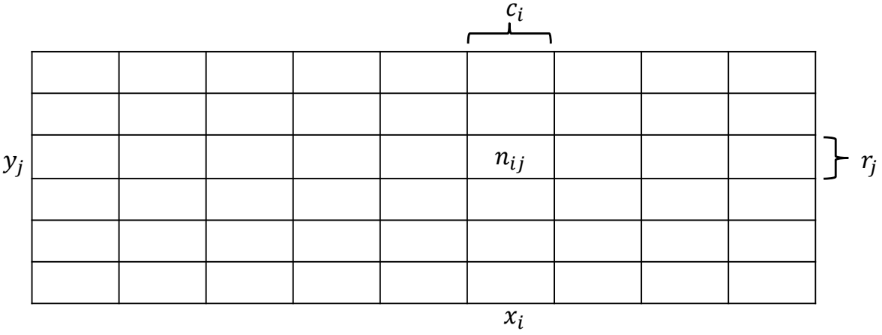
\includegraphics[width=\linewidth]{figures/summenregel.png}

\begin{itemize}
	\item Angenommen $ p(X = x_i, Y = y_j) = \frac{n_{ij}}{N} $ ist bekannt.
	\item Es gilt
	\begin{align*}
		p(X = x_i) &= \frac{c_i}{N} \\
		&= \sum_j \frac{n_{ij}}{N}
	\end{align*}
	und damit
	\begin{align*}
		p(X = x_i) &= \sum_j \frac{n_{ij}}{N} \\
		&= \sum_j p(X = x_i, Y = y_j)
	\end{align*}
\end{itemize}

\subsubsection{Produktregel (Wahrscheinlichkeit)}

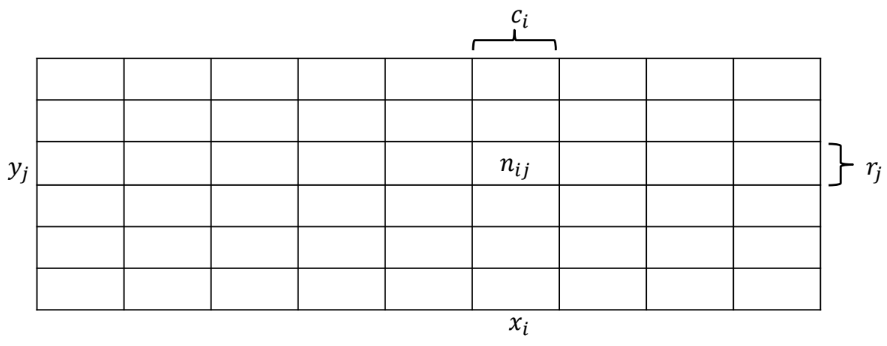
\includegraphics[width=\linewidth]{figures/produktregel.png}

\begin{itemize}
	\item Tatsächlich ist bekannt: $ p(Y = y_j \mid X = x_i) = 
	\frac{n_{ij}}{c_i} $.
	\item Ferner ist bekannt: $ p(X = x_i) = \frac{c_i}{N} $.
	\item Daraus ergibt sich
	\begin{align*}
		p(X = x_i, Y = y_j) &= \frac{n_{ij}}{N} \\
		&= \frac{n_{ij}}{c_i} \cdot \frac{c_i}{N}
	\end{align*}
	und somit
	\[ p(X = x_i, Y = y_j) = p(Y = y_j \mid X = x_i) p(X = x_i) \]
\end{itemize}

\begin{itemize}
	\item $ P(C) $ und $ p(x \mid C) $ können basierend auf den Daten oder 
	einer Stichprobe davon berechnet werden.
	\item $ p(x) = p(x \mid C=1) P(C=1) + p(x \mid C=0) P(C=0) $ im Fall eines 
	binären Klassifikationsproblems
	\item Im allgemeinen Fall gibt es $ k $ Klassen:
	\[ P(C_i \mid x) = \frac{P(C_i) p(x \mid C_i)}{\sum_k P(C_k) p(x \mid C_k)} 
	\]
	\item Klasse $ k $ wird gewählt, falls $ k = \arg \max_i P(C_i \mid x) $
\end{itemize}

\subsubsection{Univariater Fall}

\begin{itemize}
	\item Die Dichten der Verteilungen $ P(C_i) $ und $ p(x \mid C_i) $ müssen 
	für alle $ i $ geschätzt werden.
	\item Es kann eine (bis auf die Parameter) bekannte Verteilung vorliegen.
	\begin{itemize}
		\item Es gibt Tests, um auf eine bestimmte Verteilung hin zu testen.
		\item Es reichen jedoch auch Histrogramme und qq-Plots.
		\item Die Berechnung der unbekannten Parameter erfolgt durch 
		Optimierung (Maximum Likelihood).
	\end{itemize}
	\item Die Verteilung kann sich aus mehreren bekannten Dichten 
	zusammensetzen (z.B. Mixture of Gaussians).
	\item Wenn die Dichte nicht bekannt ist, so kann auf ein $ k $-NN oder 
	Kernel Verfahren zurückgegriffen werden.
\end{itemize}

\subsubsection{Schätzung der a-priori Wahrscheinlichkeiten}

\begin{itemize}
	\item Die a-priori Wahrscheinlichkeiten werden aus dem Datensatz geschätzt 
	mit
	\[ p(C_k) = \frac{N_k}{N} \]
	wobei $ N_k $ die Anzahl der Instanzen mit der Klassenzugehörigkeit $ k $ 
	ist und $ N $ die Anzahl der Daten im Datensatz.
\end{itemize}

\subsubsection{Dichteschätzer}

\begin{itemize}
	\item Gegeben sind unabhängige und identisch verteilte Stichproben:
	\[ X = \{ x_{i1} \}_{i=1}^N = \{ x_i \}_{i=1}^N \]
	\item Die $ x_i $ sind nach einer bis auf $ \theta $ bekannten Dichte $ p(x 
	\mid \theta) $ gezogen worden.
	\item Gefunden werden soll das $ \theta $, bei dem die $ x_i $ am 
	wahrscheinlichsten aus $ p(x \mid \theta) $ gezogen wurden.
	\item Aufgrund der iid Annahme ergibt sich die Likelihood:
	\begin{align*}
		l(\theta \mid X) &\equiv p(X \mid \theta) \\
		&= \sum_{i=1}^{N} p(x_i \mid \theta)
	\end{align*}
	\item Ziehen des Logarithmus (log-Likelihood) und Ableiten ermöglicht nun 
	das Maximieren.
\end{itemize}

\paragraph{Gauss-Verteilung}

\begin{itemize}
	\item $ p(x \mid \mu, \sigma) = \frac{1}{\sigma \sqrt{2 \pi}}^{\frac{-(x - 
	\mu)^2}{2 \sigma^2}} $
	\item Die Maximum Likelihood (ML) Schätzer sind
	\begin{align*}
		\hat{m} &= \frac{\sum_{i=1}^{N} x_i}{N} \\
		\hat{s}^2 &= \frac{\sum_{i=1}^{N} (x_i - \hat{m})^2}{N}
	\end{align*}
\end{itemize}

\paragraph{Bernoulli-Verteilung und deren Verallgemeinerung}

\begin{itemize}
	\item $ P(x \mid p) = p^x (1-p)^{1-x}, x \in \{ 0,1 \} $
	\item Der ML Schätzer ist $ \hat{p} = \frac{\sum_{i=1}^{N} x_i}{N} $
	\item Verallgemeinert auf $ k $ Zustände erhält man ($ \sum_{j=1}^{k} p_j = 
	1 $)
	\[ P(x_{i1}, \ldots, x_{ik} \mid p) = \prod_{j=1}^{k} p_j^{x_{ij}} \]
	und als ML Schätzer
	\[ \hat{p} = \frac{\sum_{i=1}^{N} x_{ij}}{N} \]
\end{itemize}

\paragraph{Binomialverteilung}

\begin{itemize}
	\item Verwandt mit dem Bernoulli Experiment
	\item $ m $ ist die Anzahl der Beobachtungen mit $ x=1 $ für ein Bernoulli 
	Experiment (bzw. die zugehörige Variable)
	\item $ Bin(m \mid N,p) = \binom{N}{m} p^m (1-p)^{N-m} $
	\item $ E(m) = Np $
	\item $ Var(m) = Np(1-p) $
\end{itemize}

\subsubsection{Verteilungen}

\begin{itemize}
	\item Setzt sich eine Verteilung aus $ n $ Verteilungen (z.B. 
	Normalverteilungen) zusammen, so gilt:
	\[ p(x) = \sum_{j=1}^{n} \pi_j \mathcal{N} (x \mid \mu_j, \sigma_j) \]
	\item $ \sum_{j=1}^{n} \pi_j = 1 $
	\item Nun sollen die Parameter $ \mu_j, \sigma_j, \pi_j, (1 \leq j \leq n) 
	$ aus den Daten geschätzt werden.
	\item Mit der log-Likelihood Methode ergibt sich:
	\[ \sum_{i=1}^{N} \log  \sum_{j=1}^{n} \pi_j \mathcal{N} (x_i \mid \mu_j, 
	\sigma_j) \rightarrow \max \]
\end{itemize}

\section{Clustering}

\section{Warenkorbanalyse}

\section{Analyse von Graphdaten}

\end{document}